\section{Технический проект}
\subsection{Архитектура программной системы}

Приложение построено по архитектуре «клиент-сервер». Серверная часть включает встроенную СУБД PostgreSQL, развёртываемую через библиотеку pgembed, и веб-сервер на основе микрофреймворка Flask. Клиентская часть представлена десктопным приложением (Tkinter) и веб-браузером, через который осуществляется основная работа с системой.

Локальное использование обосновано спецификой задачи. Для центра повышения квалификации удобно использовать локальный веб-сервер: несколько сотрудников одновременно работают с общей базой данных через браузер. Администратор, запускающий приложение, управляет сервером кнопками запуска и остановки. Остальные пользователи подключаются по локальному IP-адресу компьютера администратора на порт 5000.

Общая схема взаимодействия компонентов приложения показана на рисунке~\ref{fig:architecture}.

\begin{figure}[H]
	\center{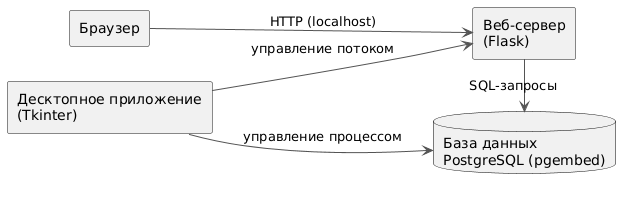
\includegraphics[width=1\linewidth]{architecture}}
	\caption{Общая схема взаимодействия компонентов}
	\label{fig:architecture}
\end{figure}

Десктопное приложение (Tkinter) отвечает за управление жизненным циклом серверной части. При запуске оно инициализирует PostgreSQL, создаёт базу данных (если она отсутствует), развёртывает структуру таблиц с помощью модуля \texttt{schema.py} и заполняет справочники начальными значениями. Затем запускается веб-сервер Flask в отдельном потоке и открывается браузер с интерфейсом приложения. При завершении работы десктопное приложение корректно останавливает веб-сервер и процесс PostgreSQL.

Серверная часть функционирует локально. Встроенная СУБД PostgreSQL использует предопределённые параметры подключения: имя пользователя — \texttt{postgres}, пароль — пустой, имя базы данных — \texttt{cpkprog\_db}. Данные физически хранятся в подкаталоге \texttt{./pgdata} каталога приложения.

\subsection{Обоснование выбора технологии проектирования}

При выборе технологического стека учитывались следующие критерии: возможность автономной работы без установки дополнительного ПО, простота развёртывания, наличие необходимых библиотек и средств для работы с базой данных и веб-интерфейсом.

\subsubsection{Язык программирования Python}

Основным языком разработки выбран Python 3.13. Данный язык предоставляет все необходимые для проекта библиотеки: psycopg2 для взаимодействия с PostgreSQL, Flask для создания веб-интерфейса, Tkinter для графического интерфейса пользователя. Ключевым преимуществом стало наличие библиотеки pgembed, которая позволяет встроить PostgreSQL непосредственно в приложение, избавляя пользователя от необходимости устанавливать и настраивать СУБД вручную. Дополнительным плюсом является кроссплатформенность Python, что при минимальных доработках позволит запускать приложение на различных операционных системах.

\subsubsection{Микрофреймворк Flask}

В качестве веб-фреймворка выбран Flask — легковесный фреймворк на языке Python, позволяющий запустить веб-сервер с минимальными усилиями. Flask не требует установки внешнего веб-сервера и обслуживает HTTP-запросы самостоятельно.

Встроенный шаблонизатор Jinja2 отделяет HTML-верстку от программной логики. В шаблонах размещаются метки-заполнители, на место которых Flask подставляет данные из базы данных — списки слушателей, названия справочников, сообщения об ошибках. Это избавляет от необходимости формировать HTML-код внутри Python-сценариев и упрощает поддержку интерфейса.

Механизм маршрутизации связывает URL-адреса с функциями-обработчиками. Например, запрос к \texttt{/add\_student} направляется к функции добавления слушателя, а запрос к \texttt{/edit\_student/5} — к функции редактирования слушателя с идентификатором 5. Параметры URL извлекаются автоматически.

Для аутентификации используется расширение Flask-Login с кастомным декоратором \texttt{@admin\_required}, проверяющим наличие у пользователя прав администратора.

Библиотека werkzeug, на которой построен Flask, предоставляет класс \texttt{make\_server}, позволяющий запустить веб-сервер в отдельном потоке внутри графического интерфейса пользователя. Это даёт возможность управлять запуском и остановкой сервера через графический интерфейс.

\subsubsection{СУБД PostgreSQL и библиотека pgembed}

В качестве системы управления базами данных выбрана PostgreSQL. Эта СУБД обеспечивает полную поддержку внешних ключей с каскадными операциями (ON DELETE CASCADE), благодаря чему при удалении слушателя автоматически удаляются все связанные записи — документы, финансирование, характеристики, предыдущее образование. Поддержка транзакций с возможностью отката гарантирует, что при сбое во время операции добавления или редактирования данные не будут частично сохранены.

Ключевым компонентом проекта является библиотека pgembed. Она встраивает PostgreSQL непосредственно в десктопное приложение: при первом запуске автоматически развёртывает экземпляр СУБД, создаёт базу данных и инициализирует структуру таблиц. Пользователю не требуется устанавливать PostgreSQL отдельно или настраивать параметры подключения.

Для эффективной работы с базой данных используется пул соединений. При запуске создаётся от 2 до 10 потокобезопасных соединений, которые переиспользуются между запросами. Это исключает накладные расходы на постоянное открытие и закрытие подключений и позволяет обслуживать несколько одновременных запросов от разных вкладок браузера.

\subsubsection{Библиотека Tkinter}

Графический интерфейс пользователя реализован на библиотеке Tkinter. Она входит в стандартную поставку Python, поэтому не требует установки дополнительных зависимостей и не увеличивает размер дистрибутива. Функциональности Tkinter достаточно для создания интерфейса с кнопками управления сервером, отображения статуса, а также дополнительных окон для просмотра статистики, журнала событий и выбора файла импорта.

\subsubsection{Прочие библиотеки}

Для чтения и обработки Excel-файлов при импорте данных используется библиотека pandas. Хеширование паролей пользователей выполняется средствами werkzeug (\texttt{generate\_password\_hash}, \texttt{check\_password\_hash}). Логирование событий приложения реализовано стандартным модулем Python logging с записью в файл \texttt{app.log} и дублированием в консоль.


\subsection{Клиентская часть}

Клиентская часть включает десктопное приложение на Tkinter и браузеры пользователей. Десктопное приложение предоставляет графический интерфейс для управления сервером и дополнительные функции, не связанные напрямую с веб-интерфейсом. На рисунке~\ref{fig:client_comp} приведена диаграмма компонентов клиентской части.

\begin{figure}[H]
	\center{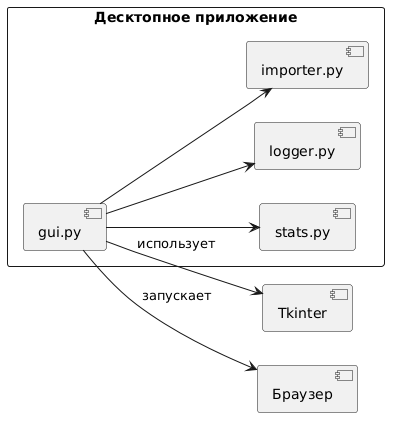
\includegraphics[width=0.65\linewidth]{client_component}}
	\caption{Диаграмма компонентов клиентской части}
	\label{fig:client_comp}
\end{figure}

Внешней платформой для десктопного приложения является библиотека Tkinter, обеспечивающая создание окон, кнопок и других элементов интерфейса. Основным компонентом является \texttt{gui.py} — главное окно приложения. Оно содержит кнопки «Запустить сервер» и «Остановить сервер», статусную строку, а также кнопки вызова дополнительных функций: «Статистика», «Журнал событий», «Загрузить из Excel», «Пользователи».

При нажатии на кнопку запуска \texttt{gui.py} выполняет последовательную инициализацию: запускает процесс PostgreSQL через \texttt{connection.py}, создаёт базу данных и таблицы через \texttt{schema.py}, запускает веб-сервер Flask в отдельном потоке и открывает браузер. При остановке последовательно завершает работу Flask, закрывает пул соединений и останавливает PostgreSQL.

Модуль \texttt{stats.py} вызывается при нажатии кнопки «Статистика». Он выполняет несколько SQL-запросов к базе данных и формирует текстовый отчёт, который отображается в отдельном окне Tkinter с возможностью копирования в буфер обмена.

Модуль \texttt{logger.py} обеспечивает просмотр и очистку журнала событий. Кнопка «Журнал событий» открывает окно, в которое загружается содержимое файла \texttt{app.log}. Пользователь может обновить содержимое или полностью очистить файл.

Модуль \texttt{importer.py} реализует импорт данных из Excel-файлов. По нажатию кнопки «Загрузить из Excel» открывается стандартный диалог выбора файла, после чего модуль считывает данные, выполняет сопоставление столбцов, валидацию и вставку записей в базу данных.

Все перечисленные модули клиентской части не зависят от веб-сервера Flask и взаимодействуют с базой данных напрямую через \texttt{connection.py}.

\subsection{Серверная часть}

Серверная часть реализует веб-интерфейс системы и содержит всю бизнес-логику обработки данных. На рисунке~\ref{fig:server_comp} представлена диаграмма компонентов серверной части.

\begin{figure}[H]
	\center{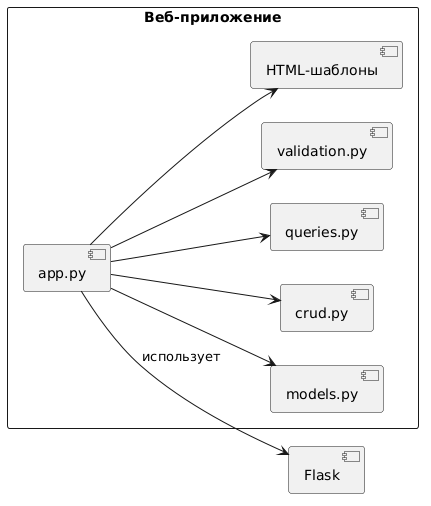
\includegraphics[width=0.6\linewidth]{server_component}}
	\caption{Диаграмма компонентов серверной части}
	\label{fig:server_comp}
\end{figure}

Внешней средой для серверной части является веб-фреймворк Flask, предоставляющий маршрутизацию, обработку запросов и шаблонизатор Jinja2. Центральный компонент \texttt{app.py} определяет все маршруты: для работы со слушателями (\texttt{/}, \texttt{/add\_student}, \texttt{/edit\_student/<id>}, \texttt{/delete\_student/<id>}), аутентификации (\texttt{/login}, \texttt{/logout}) и управления пользователями (\texttt{/admin/users}).

Аутентификация реализована с помощью расширения Flask-Login. При входе вызывается \texttt{login\_user}, создающая защищённую сессию. При каждом запросе Flask-Login автоматически загружает пользователя через функцию \texttt{load\_user} и предоставляет объект \texttt{current\_user}. Проверка прав администратора выполняется декоратором \texttt{@admin\_required}.

Модель \texttt{User} (\texttt{models.py}) наследуется от \texttt{UserMixin} и содержит методы поиска пользователя и проверки пароля.

Модуль \texttt{crud.py} отвечает за вставку и обновление записей о слушателях в рамках одной транзакции, охватывающей все связанные таблицы. Модуль \texttt{queries.py} формирует SQL-запросы с JOIN к тринадцати таблицам и динамической фильтрацией. Модуль \texttt{validation.py} проверяет корректность полей: формат СНИЛС, телефона, дат, согласованность дат и т.д.

\subsubsection{Обработка запроса}
На рисунке~\ref{fig:sequence} приведена диаграмма последовательности, иллюстрирующая взаимодействие компонентов при обработке HTTP-запроса на добавление слушателя.

\begin{figure}[H]
	\center{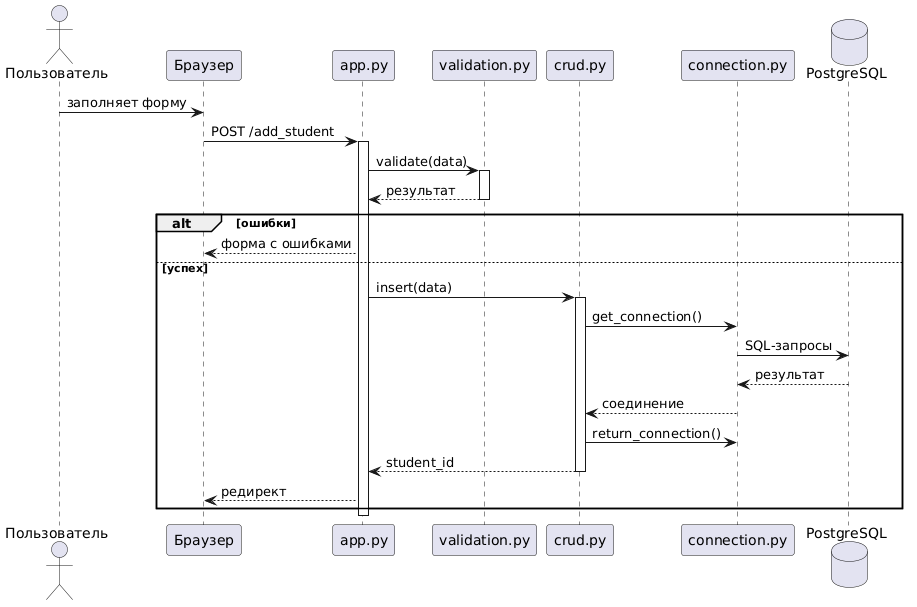
\includegraphics[width=0.9\linewidth]{sequence}}
	\caption{Диаграмма последовательности обработки запроса}
	\label{fig:sequence}
\end{figure}

Пользователь через браузер отправляет POST-запрос с данными формы. Flask-приложение получает запрос, извлекает данные и передаёт их модулю валидации. При успешной проверке данные направляются в \texttt{crud.py}, который через \texttt{connection.py} выполняет серию SQL-команд. Результат возвращается Flask, который генерирует HTML-ответ с помощью Jinja2 и отправляет его браузеру.

\subsubsection{Форматы данных}
Обмен данными между браузером и веб-сервером ведётся по протоколу HTTP. Данные форм передаются в кодировке \texttt{application/x-www-form-urlencoded}. Результаты выборок из базы данных передаются в шаблоны Jinja2 как структуры Python (списки, словари) и преобразуются в HTML на стороне сервера. Импортируемые файлы имеют формат XLSX. Журнал событий ведётся в текстовом виде с временной меткой.

\subsubsection{Программный интерфейс (API)}
В таблице~\ref{tab:api} приведены основные HTTP-запросы, обрабатываемые серверной частью. Все POST-запросы принимают данные HTML-форм в кодировке \texttt{application/x-www-form-urlencoded}.

\begin{xltabular}{\textwidth}{|c|c|>{\raggedright\arraybackslash}p{3.5cm}|X|}
	\caption{Основные HTTP-запросы серверной части\label{tab:api}}\\ \hline
	\centrow Маршрут & \centrow Метод & \centrow Входные данные & \centrow Результат \\ \hline
	\endfirsthead
	\continuecaption{Продолжение таблицы \ref{tab:api}}
	\centrow Маршрут & \centrow Метод & \centrow Входные данные & \centrow Результат \\ \hline
	\finishhead
	\texttt{/} & GET & Параметры фильтрации в URL & HTML-страница со списком слушателей \\ \hline
	\texttt{/login} & GET, POST & \texttt{username}, \texttt{password} & Вход в систему или страница с ошибкой \\ \hline
	\texttt{/logout} & GET & --- & Выход из системы \\ \hline
	\texttt{/add\_student} & GET, POST & Поля формы слушателя (45 полей) & Добавление записи или форма с ошибками \\ \hline
	\texttt{/edit\_student/<id>} & GET, POST & \texttt{id} в URL + поля формы & Обновление записи или форма с ошибками \\ \hline
	\texttt{/delete\_student/<id>} & GET & \texttt{id} в URL & Удаление записи \\ \hline
	\texttt{/admin/users} & GET & --- & Список пользователей \\ \hline
	\texttt{/admin/users/add} & GET, POST & \texttt{username}, \texttt{password}, \texttt{is\_admin} & Создание пользователя или форма с ошибкой \\ \hline
	\texttt{/admin/users/edit/<id>} & GET, POST & \texttt{id} в URL + \texttt{username}, \texttt{password}, \texttt{is\_admin} & Обновление пользователя или форма с ошибкой \\ \hline
	\texttt{/admin/users/delete/<id>} & GET & \texttt{id} в URL & Удаление пользователя \\ \hline
\end{xltabular}

В качестве примера обработки POST-запроса ниже показан маршрут добавления слушателя (\texttt{/add\_student}). Когда пользователь заполнил форму и нажал «Сохранить», браузер отправляет на сервер строку следующего вида (значения полей взяты для примера):


\begin{verbatim}
	last_name=Иванов&first_name=Пётр&patronymic=Сергеевич&
	birth_date=1990-01-01&gender=Муж&snils=123-456-789 00&
	phone=+7-999-123-45-67&citizenship_code=643&
	status_id=1&is_pedagogical=Нет&is_manager=Нет&
	group_code=ПИ-23&program_type_id=1&program_name=Python&
	department_name=Кафедра ПИ&learning_form_id=1&
	uses_dot=t&duration_hours=72&start_date=2025-09-01&...
\end{verbatim}

Flask автоматически преобразует строку от браузера в объект request.form (словарь Python). Вся дальнейшая обработка — валидация, сохранение, возврат в шаблон — работает уже с этим словарём, без разбора сырой строки. При успешной валидации программа добавляет нового слушателя в базу данных и отправляет браузеру HTTP-редирект на главную страницу, которая загружается с обновлённым списком. Если валидация обнаружила ошибки, программа возвращает ту же страницу с формой и сообщениями об ошибках.

Аналогично устроены все POST-маршруты: \texttt{/edit\_student/<id>} и \texttt{/admin/users/...}. Маршруты с методом GET либо отдают готовую HTML-страницу, либо выполняют действие (удаление) и делают редирект.

\subsubsection{Взаимодействие с базой данных}

Программные компоненты, отвечающие за управление встроенной СУБД и доступ к данным, функционируют на стороне сервера. Их состав и связи показаны на рисунке~\ref{fig:db_comp}.

\begin{figure}[H]
	\center{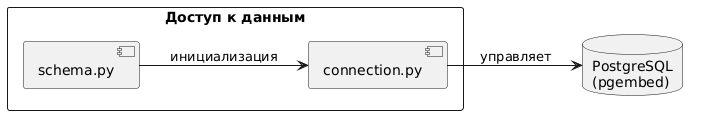
\includegraphics[scale=0.7]{db_component}}
	\caption{Программные компоненты взаимодействия с СУБД}
	\label{fig:db_comp}
\end{figure}

Модуль \texttt{connection.py} управляет процессом PostgreSQL, создаёт пул соединений \texttt{ThreadedConnectionPool} (от 2 до 10 потокобезопасных соединений) и предоставляет методы \texttt{get\_connection()} и \texttt{return\_connection()} для остальных модулей.

Модуль \texttt{schema.py} вызывается однократно при первом запуске и выполняет создание всех таблиц, заполнение справочников и создание учётной записи администратора.

Физически данные хранятся в подкаталоге \texttt{./pgdata} каталога приложения. При повторных запусках инициализация пропускается.

\subsection{Проект базы данных программно-информационной системы}

\subsubsection{Концептуальная модель данных}

На основе анализа предметной области были выделены основные сущности и связи между ними. ER-диаграмма (Entity-Relationship diagram, диаграмма «сущность-связь») представляет собой графическую схему, которая показывает, какие данные присутствуют в системе и как они связаны друг с другом. На рисунке \ref{er:image} представлена концептуальная модель данных.

\begin{figure}[H]
	\center{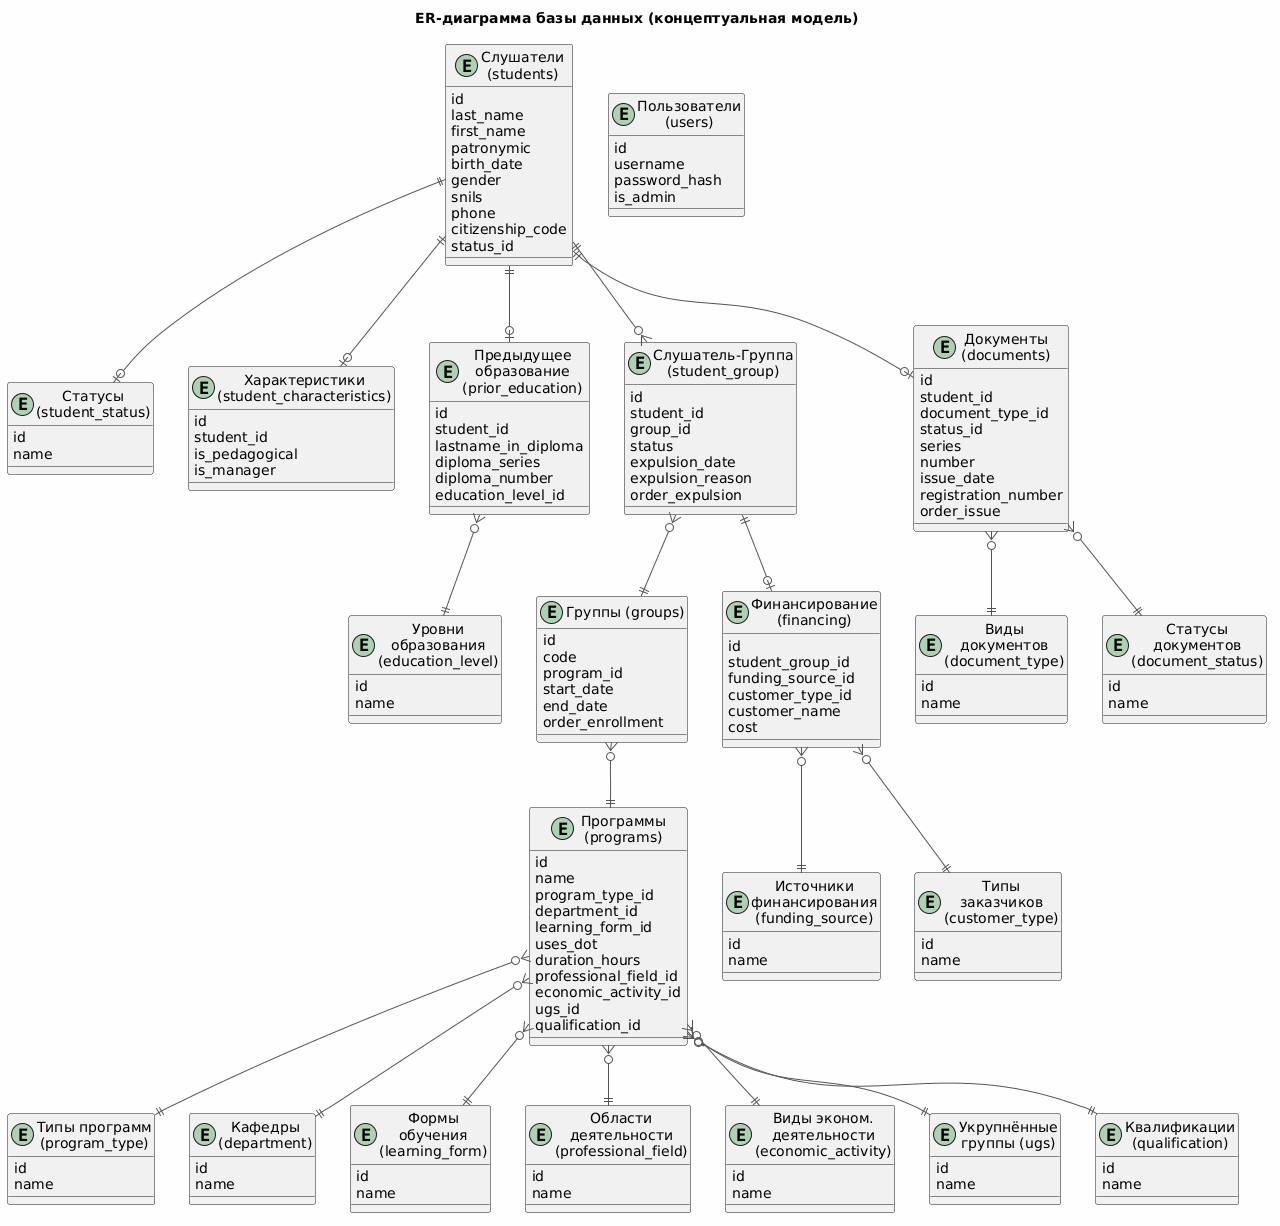
\includegraphics[width=1\linewidth]{er}}
	\caption{Концептуальная модель данных}
	\label{er:image}
\end{figure}

\subsubsection{Нормализация}

Схема базы данных спроектирована в соответствии с требованиями третьей нормальной формы. Все атрибуты атомарны, каждая таблица имеет суррогатный первичный ключ, ссылки на справочные таблицы реализованы через внешние ключи, связующие таблицы вынесены в отдельные сущности. Транзитивные зависимости отсутствуют.

\subsubsection{Реляционная модель данных}

На основе ER-модели построена реляционная модель данных. На рисунке \ref{rel:image} представлена схема базы данных.

\begin{figure}[H]
	\center{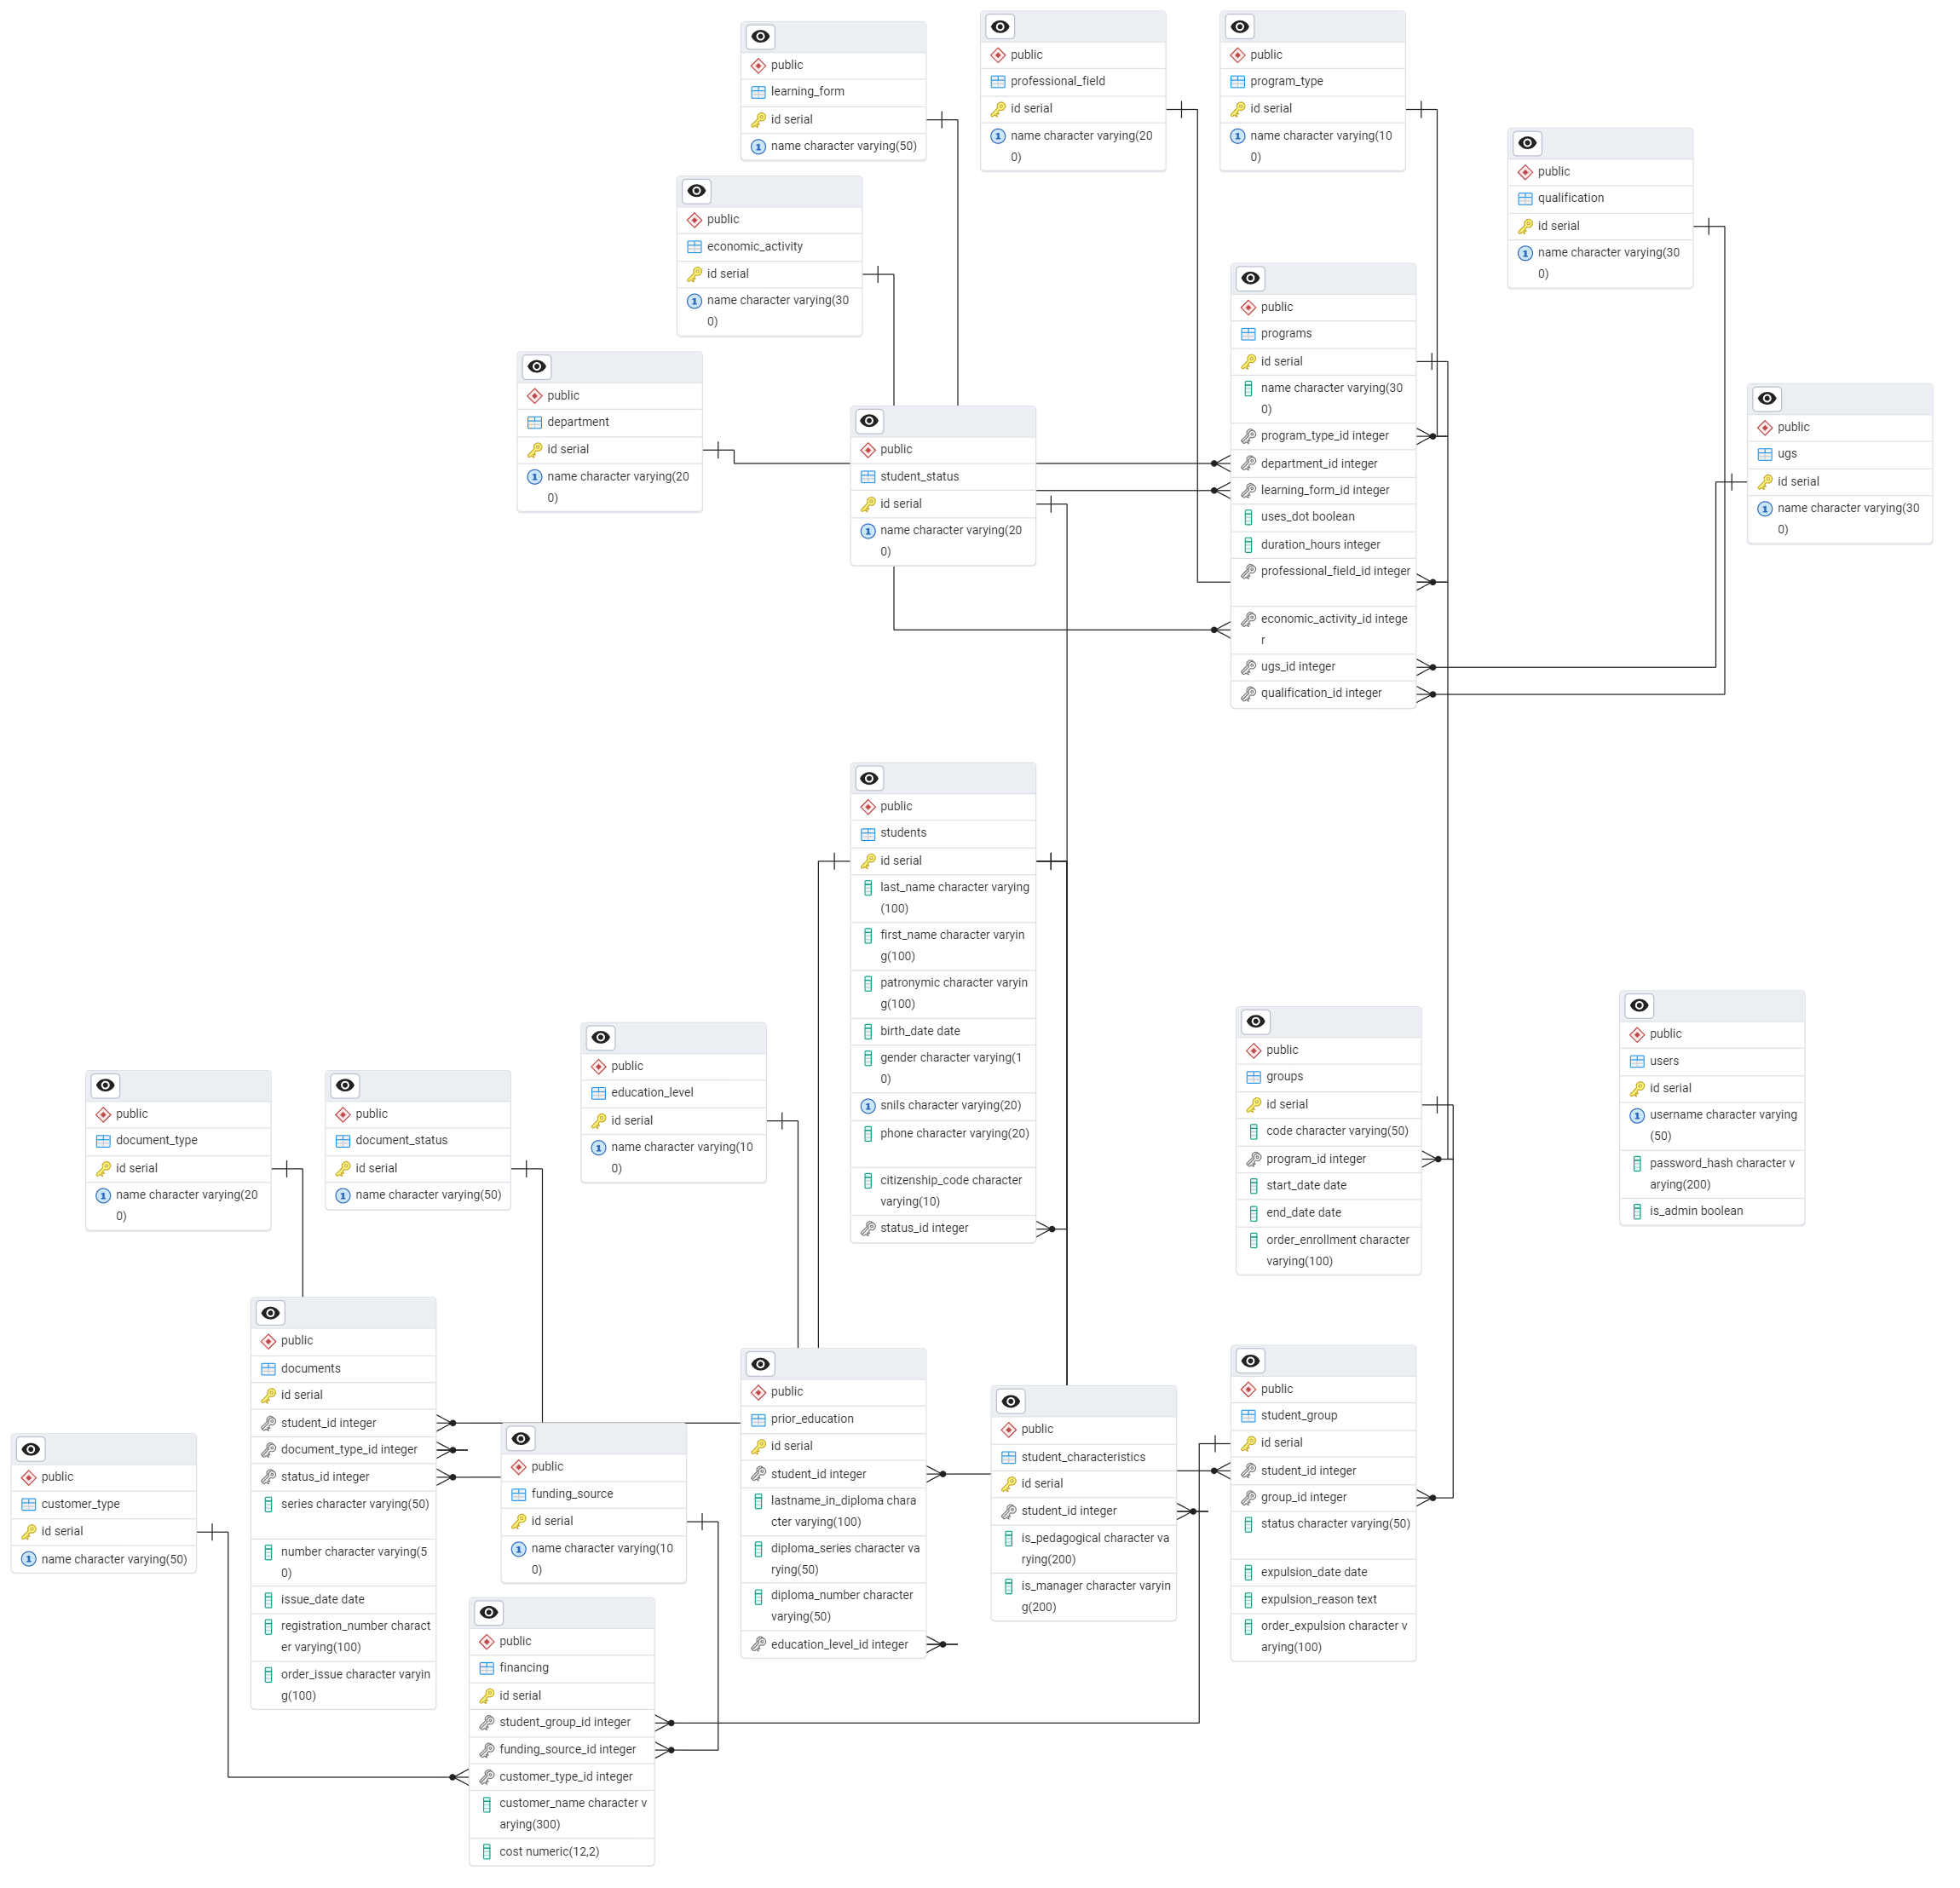
\includegraphics[scale=0.2]{rel}}
	\caption{Реляционная модель данных}
	\label{rel:image}
\end{figure}

\subsubsection{Описание структуры базы данных}

В таблицах \ref{tab:students}--\ref{tab:users} приведено описание структуры таблиц базы данных.

\begin{xltabular}{\textwidth}{|c|c|l|l|X|}
	\caption{Схема таблицы «students» (Слушатели)\label{tab:students}}\\ \hline
	\centrow Key Type & \centrow Optionality & \centrow Column name & \centrow Data Type & \centrow Size \\ \hline
	\endfirsthead
	\continuecaption{Продолжение таблицы \ref{tab:students}}
	\centrow Key Type & \centrow Optionality & \centrow Column name & \centrow Data Type & \centrow Size \\ \hline
	\finishhead
	PK & * & id & SERIAL & \\ \hline
	& * & last\_name & VARCHAR & 100 \\ \hline
	& * & first\_name & VARCHAR & 100 \\ \hline
	& & patronymic & VARCHAR & 100 \\ \hline
	& * & birth\_date & DATE & dd/mm/yyyy \\ \hline
	& & gender & VARCHAR & 10 \\ \hline
	UK & & snils & VARCHAR & 20 \\ \hline
	& & phone & VARCHAR & 20 \\ \hline
	& & citizenship\_code & VARCHAR & 10 \\ \hline
	FK & & status\_id & INTEGER & \\ \hline
\end{xltabular}

\begin{xltabular}{\textwidth}{|c|c|l|l|X|}
	\caption{Схема таблицы «student\_status» (Статусы слушателей)\label{tab:student_status}}\\ \hline
	\centrow Key Type & \centrow Optionality & \centrow Column name & \centrow Data Type & \centrow Size \\ \hline
	\endfirsthead
	\continuecaption{Продолжение таблицы \ref{tab:student_status}}
	\centrow Key Type & \centrow Optionality & \centrow Column name & \centrow Data Type & \centrow Size \\ \hline
	\finishhead
	PK & * & id & SERIAL & \\ \hline
	UK & * & name & VARCHAR & 200 \\ \hline
\end{xltabular}

\begin{xltabular}{\textwidth}{|c|c|l|l|X|}
	\caption{Атрибуты таблицы «student\_characteristics» (Характеристики слушателя)\label{tab:characteristics}}\\ \hline
	\centrow Key Type & \centrow Optionality & \centrow Column name & \centrow Data Type & \centrow Size \\ \hline
	\endfirsthead
	\continuecaption{Продолжение таблицы \ref{tab:characteristics}}
	\centrow Key Type & \centrow Optionality & \centrow Column name & \centrow Data Type & \centrow Size \\ \hline
	\finishhead
	PK & * & id & SERIAL & \\ \hline
	FK & * & student\_id & INTEGER & \\ \hline
	& & is\_pedagogical & VARCHAR & 200 \\ \hline
	& & is\_manager & VARCHAR & 200 \\ \hline
\end{xltabular}

\begin{xltabular}{\textwidth}{|c|c|l|l|X|}
	\caption{Схема таблицы «prior\_education» (Предыдущее образование)\label{tab:prior_education}}\\ \hline
	\centrow Key Type & \centrow Optionality & \centrow Column name & \centrow Data Type & \centrow Size \\ \hline
	\endfirsthead
	\continuecaption{Продолжение таблицы \ref{tab:prior_education}}
	\centrow Key Type & \centrow Optionality & \centrow Column name & \centrow Data Type & \centrow Size \\ \hline
	\finishhead
	PK & * & id & SERIAL & \\ \hline
	FK & * & student\_id & INTEGER & \\ \hline
	& & lastname\_in\_diploma & VARCHAR & 100 \\ \hline
	& & diploma\_series & VARCHAR & 50 \\ \hline
	& & diploma\_number & VARCHAR & 50 \\ \hline
	FK & & education\_level\_id & INTEGER & \\ \hline
\end{xltabular}

\begin{xltabular}{\textwidth}{|c|c|l|l|X|}
	\caption{Схема таблицы «education\_level» (Уровни образования)\label{tab:education_level}}\\ \hline
	\centrow Key Type & \centrow Optionality & \centrow Column name & \centrow Data Type & \centrow Size \\ \hline
	\endfirsthead
	\continuecaption{Продолжение таблицы \ref{tab:education_level}}
	\centrow Key Type & \centrow Optionality & \centrow Column name & \centrow Data Type & \centrow Size \\ \hline
	\finishhead
	PK & * & id & SERIAL & \\ \hline
	UK & * & name & VARCHAR & 100 \\ \hline
\end{xltabular}

\begin{xltabular}{\textwidth}{|c|c|l|l|X|}
	\caption{Схема таблицы «student\_group» (Связь слушателей с группами)\label{tab:student_group}}\\ \hline
	\centrow Key Type & \centrow Optionality & \centrow Column name & \centrow Data Type & \centrow Size \\ \hline
	\endfirsthead
	\continuecaption{Продолжение таблицы \ref{tab:student_group}}
	\centrow Key Type & \centrow Optionality & \centrow Column name & \centrow Data Type & \centrow Size \\ \hline
	\finishhead
	PK & * & id & SERIAL & \\ \hline
	FK & * & student\_id & INTEGER & \\ \hline
	FK & * & group\_id & INTEGER & \\ \hline
	& & status & VARCHAR & 50 \\ \hline
	& & expulsion\_date & DATE & dd/mm/yyyy \\ \hline
	& & expulsion\_reason & TEXT & \\ \hline
	& & order\_expulsion & VARCHAR & 100 \\ \hline
\end{xltabular}

\begin{xltabular}{\textwidth}{|c|c|l|l|X|}
	\caption{Схема таблицы «groups» (Группы)\label{tab:groups}}\\ \hline
	\centrow Key Type & \centrow Optionality & \centrow Column name & \centrow Data Type & \centrow Size \\ \hline
	\endfirsthead
	\continuecaption{Продолжение таблицы \ref{tab:groups}}
	\centrow Key Type & \centrow Optionality & \centrow Column name & \centrow Data Type & \centrow Size \\ \hline
	\finishhead
	PK & * & id & SERIAL & \\ \hline
	& * & code & VARCHAR & 50 \\ \hline
	FK & & program\_id & INTEGER & \\ \hline
	& & start\_date & DATE & dd/mm/yyyy \\ \hline
	& & end\_date & DATE & dd/mm/yyyy \\ \hline
	& & order\_enrollment & VARCHAR & 100 \\ \hline
\end{xltabular}

\begin{xltabular}{\textwidth}{|c|c|l|l|X|}
	\caption{Схема таблицы «programs» (Программы обучения)\label{tab:programs}}\\ \hline
	\centrow Key Type & \centrow Optionality & \centrow Column name & \centrow Data Type & \centrow Size \\ \hline
	\endfirsthead
	\continuecaption{Продолжение таблицы \ref{tab:programs}}
	\centrow Key Type & \centrow Optionality & \centrow Column name & \centrow Data Type & \centrow Size \\ \hline
	\finishhead
	PK & * & id & SERIAL & \\ \hline
	& * & name & VARCHAR & 300 \\ \hline
	FK & & program\_type\_id & INTEGER & \\ \hline
	FK & & department\_id & INTEGER & \\ \hline
	FK & & learning\_form\_id & INTEGER & \\ \hline
	& & uses\_dot & BOOLEAN & \\ \hline
	& & duration\_hours & INTEGER & \\ \hline
	FK & & professional\_field\_id & INTEGER & \\ \hline
	FK & & economic\_activity\_id & INTEGER & \\ \hline
	FK & & ugs\_id & INTEGER & \\ \hline
	FK & & qualification\_id & INTEGER & \\ \hline
\end{xltabular}

\begin{xltabular}{\textwidth}{|c|c|l|l|X|}
	\caption{Схема таблицы «program\_type» (Типы программ)\label{tab:program_type}}\\ \hline
	\centrow Key Type & \centrow Optionality & \centrow Column name & \centrow Data Type & \centrow Size \\ \hline
	\endfirsthead
	\continuecaption{Продолжение таблицы \ref{tab:program_type}}
	\centrow Key Type & \centrow Optionality & \centrow Column name & \centrow Data Type & \centrow Size \\ \hline
	\finishhead
	PK & * & id & SERIAL & \\ \hline
	UK & * & name & VARCHAR & 100 \\ \hline
\end{xltabular}

\begin{xltabular}{\textwidth}{|c|c|l|l|X|}
	\caption{Схема таблицы «department» (Кафедры)\label{tab:department}}\\ \hline
	\centrow Key Type & \centrow Optionality & \centrow Column name & \centrow Data Type & \centrow Size \\ \hline
	\endfirsthead
	\continuecaption{Продолжение таблицы \ref{tab:department}}
	\centrow Key Type & \centrow Optionality & \centrow Column name & \centrow Data Type & \centrow Size \\ \hline
	\finishhead
	PK & * & id & SERIAL & \\ \hline
	UK & * & name & VARCHAR & 200 \\ \hline
\end{xltabular}

\begin{xltabular}{\textwidth}{|c|c|l|l|X|}
	\caption{Схема таблицы «learning\_form» (Формы обучения)\label{tab:learning_form}}\\ \hline
	\centrow Key Type & \centrow Optionality & \centrow Column name & \centrow Data Type & \centrow Size \\ \hline
	\endfirsthead
	\continuecaption{Продолжение таблицы \ref{tab:learning_form}}
	\centrow Key Type & \centrow Optionality & \centrow Column name & \centrow Data Type & \centrow Size \\ \hline
	\finishhead
	PK & * & id & SERIAL & \\ \hline
	UK & * & name & VARCHAR & 50 \\ \hline
\end{xltabular}

\begin{xltabular}{\textwidth}{|c|c|l|l|X|}
	\caption{Схема таблицы «professional\_field» (Области профессиональной деятельности)\label{tab:professional_field}}\\ \hline
	\centrow Key Type & \centrow Optionality & \centrow Column name & \centrow Data Type & \centrow Size \\ \hline
	\endfirsthead
	\continuecaption{Продолжение таблицы \ref{tab:professional_field}}
	\centrow Key Type & \centrow Optionality & \centrow Column name & \centrow Data Type & \centrow Size \\ \hline
	\finishhead
	PK & * & id & SERIAL & \\ \hline
	UK & * & name & VARCHAR & 200 \\ \hline
\end{xltabular}

\begin{xltabular}{\textwidth}{|c|c|l|l|X|}
	\caption{Схема таблицы «economic\_activity» (Виды экономической деятельности)\label{tab:economic_activity}}\\ \hline
	\centrow Key Type & \centrow Optionality & \centrow Column name & \centrow Data Type & \centrow Size \\ \hline
	\endfirsthead
	\continuecaption{Продолжение таблицы \ref{tab:economic_activity}}
	\centrow Key Type & \centrow Optionality & \centrow Column name & \centrow Data Type & \centrow Size \\ \hline
	\finishhead
	PK & * & id & SERIAL & \\ \hline
	UK & * & name & VARCHAR & 300 \\ \hline
\end{xltabular}

\begin{xltabular}{\textwidth}{|c|c|l|l|X|}
	\caption{Схема таблицы «ugs» (Укрупнённые группы специальностей)\label{tab:ugs}}\\ \hline
	\centrow Key Type & \centrow Optionality & \centrow Column name & \centrow Data Type & \centrow Size \\ \hline
	\endfirsthead
	\continuecaption{Продолжение таблицы \ref{tab:ugs}}
	\centrow Key Type & \centrow Optionality & \centrow Column name & \centrow Data Type & \centrow Size \\ \hline
	\finishhead
	PK & * & id & SERIAL & \\ \hline
	UK & * & name & VARCHAR & 300 \\ \hline
\end{xltabular}

\begin{xltabular}{\textwidth}{|c|c|l|l|X|}
	\caption{Схема таблицы «qualification» (Квалификации)\label{tab:qualification}}\\ \hline
	\centrow Key Type & \centrow Optionality & \centrow Column name & \centrow Data Type & \centrow Size \\ \hline
	\endfirsthead
	\continuecaption{Продолжение таблицы \ref{tab:qualification}}
	\centrow Key Type & \centrow Optionality & \centrow Column name & \centrow Data Type & \centrow Size \\ \hline
	\finishhead
	PK & * & id & SERIAL & \\ \hline
	UK & * & name & VARCHAR & 300 \\ \hline
\end{xltabular}

\begin{xltabular}{\textwidth}{|c|c|l|l|X|}
	\caption{Схема таблицы «financing» (Финансирование)\label{tab:financing}}\\ \hline
	\centrow Key Type & \centrow Optionality & \centrow Column name & \centrow Data Type & \centrow Size \\ \hline
	\endfirsthead
	\continuecaption{Продолжение таблицы \ref{tab:financing}}
	\centrow Key Type & \centrow Optionality & \centrow Column name & \centrow Data Type & \centrow Size \\ \hline
	\finishhead
	PK & * & id & SERIAL & \\ \hline
	FK & * & student\_group\_id & INTEGER & \\ \hline
	FK & & funding\_source\_id & INTEGER & \\ \hline
	FK & & customer\_type\_id & INTEGER & \\ \hline
	& & customer\_name & VARCHAR & 300 \\ \hline
	& & cost & NUMERIC & 12,2 \\ \hline
\end{xltabular}

\begin{xltabular}{\textwidth}{|c|c|l|l|X|}
	\caption{Схема таблицы «funding\_source» (Источники финансирования)\label{tab:funding_source}}\\ \hline
	\centrow Key Type & \centrow Optionality & \centrow Column name & \centrow Data Type & \centrow Size \\ \hline
	\endfirsthead
	\continuecaption{Продолжение таблицы \ref{tab:funding_source}}
	\centrow Key Type & \centrow Optionality & \centrow Column name & \centrow Data Type & \centrow Size \\ \hline
	\finishhead
	PK & * & id & SERIAL & \\ \hline
	UK & * & name & VARCHAR & 100 \\ \hline
\end{xltabular}

\begin{xltabular}{\textwidth}{|c|c|l|l|X|}
	\caption{Схема таблицы «customer\_type» (Типы заказчиков)\label{tab:customer_type}}\\ \hline
	\centrow Key Type & \centrow Optionality & \centrow Column name & \centrow Data Type & \centrow Size \\ \hline
	\endfirsthead
	\continuecaption{Продолжение таблицы \ref{tab:customer_type}}
	\centrow Key Type & \centrow Optionality & \centrow Column name & \centrow Data Type & \centrow Size \\ \hline
	\finishhead
	PK & * & id & SERIAL & \\ \hline
	UK & * & name & VARCHAR & 50 \\ \hline
\end{xltabular}

\begin{xltabular}{\textwidth}{|c|c|l|l|X|}
	\caption{Схема таблицы «documents» (Документы о квалификации)\label{tab:documents}}\\ \hline
	\centrow Key Type & \centrow Optionality & \centrow Column name & \centrow Data Type & \centrow Size \\ \hline
	\endfirsthead
	\continuecaption{Продолжение таблицы \ref{tab:documents}}
	\centrow Key Type & \centrow Optionality & \centrow Column name & \centrow Data Type & \centrow Size \\ \hline
	\finishhead
	PK & * & id & SERIAL & \\ \hline
	FK & * & student\_id & INTEGER & \\ \hline
	FK & & document\_type\_id & INTEGER & \\ \hline
	FK & & status\_id & INTEGER & \\ \hline
	& & series & VARCHAR & 50 \\ \hline
	& & number & VARCHAR & 50 \\ \hline
	& & issue\_date & DATE & dd/mm/yyyy \\ \hline
	& & registration\_number & VARCHAR & 100 \\ \hline
	& & order\_issue & VARCHAR & 100 \\ \hline
\end{xltabular}

\begin{xltabular}{\textwidth}{|c|c|l|l|X|}
	\caption{Схема таблицы «document\_type» (Виды документов)\label{tab:document_type}}\\ \hline
	\centrow Key Type & \centrow Optionality & \centrow Column name & \centrow Data Type & \centrow Size \\ \hline
	\endfirsthead
	\continuecaption{Продолжение таблицы \ref{tab:document_type}}
	\centrow Key Type & \centrow Optionality & \centrow Column name & \centrow Data Type & \centrow Size \\ \hline
	\finishhead
	PK & * & id & SERIAL & \\ \hline
	UK & * & name & VARCHAR & 200 \\ \hline
\end{xltabular}

\begin{xltabular}{\textwidth}{|c|c|l|l|X|}
	\caption{Схема таблицы «document\_status» (Статусы документов)\label{tab:document_status}}\\ \hline
	\centrow Key Type & \centrow Optionality & \centrow Column name & \centrow Data Type & \centrow Size \\ \hline
	\endfirsthead
	\continuecaption{Продолжение таблицы \ref{tab:document_status}}
	\centrow Key Type & \centrow Optionality & \centrow Column name & \centrow Data Type & \centrow Size \\ \hline
	\finishhead
	PK & * & id & SERIAL & \\ \hline
	UK & * & name & VARCHAR & 50 \\ \hline
\end{xltabular}

\begin{xltabular}{\textwidth}{|c|c|l|l|X|}
	\caption{Схема таблицы «users» (Пользователи системы)\label{tab:users}}\\ \hline
	\centrow Key Type & \centrow Optionality & \centrow Column name & \centrow Data Type & \centrow Size \\ \hline
	\endfirsthead
	\continuecaption{Продолжение таблицы \ref{tab:users}}
	\centrow Key Type & \centrow Optionality & \centrow Column name & \centrow Data Type & \centrow Size \\ \hline
	\finishhead
	PK & * & id & SERIAL & \\ \hline
	UK & * & username & VARCHAR & 50 \\ \hline
	& * & password\_hash & VARCHAR & 200 \\ \hline
	& & is\_admin & BOOLEAN & \\ \hline
\end{xltabular}